\begin{figure}
    \centering

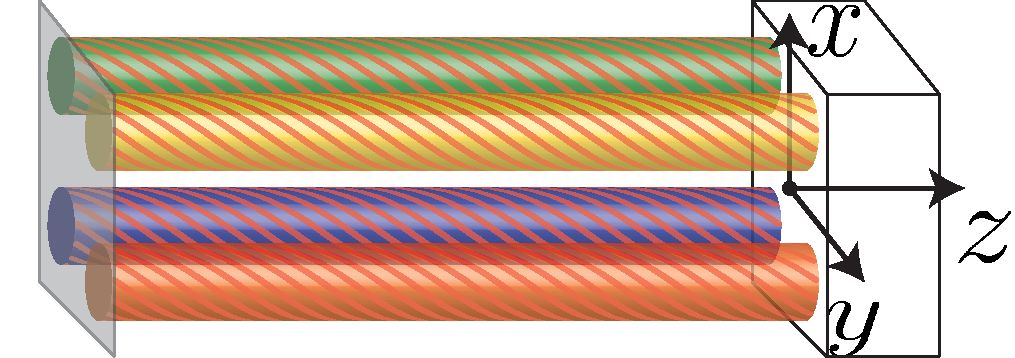
\includegraphics[width=0.6\linewidth]{figures/axesNaligned_4par-v2.pdf}

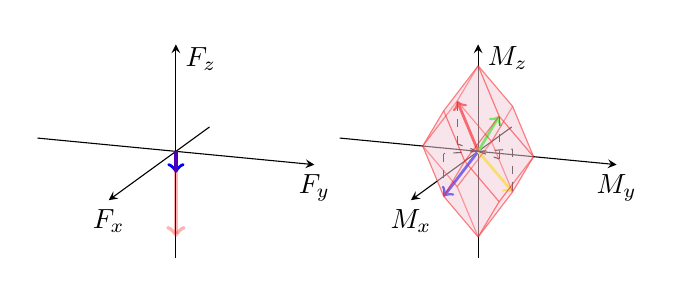
\begin{tikzpicture}
\def\scl{0.7} % define scale variable for plots

% PRACTICE PLOT
\matrix [row sep=0cm, column sep=0cm, style={align=center}] (my matrix) at (0,0)
{
% PRACTICE PLOT #3
\begin{axis}[
    view={110}{20},
    axis lines=center,
    % axis equal image,
    xlabel={$F_x$},
    ylabel={$F_y$},
    zlabel={$F_z$},
    ymin=-5, ymax=5, ytick={0}, %ylabel near ticks,
    xmin=-5, xmax=10, xtick={0}, %xticklabel=$\pgfmathprintnumber{\tick}^\circ$, xlabel near ticks, 
    zmin=-5, zmax=5, ztick={0}, %z dir=reverse,
    xlabel style={anchor=north}, ylabel style={anchor=north},
    scale=\scl,
    anchor=center,
    ]
    \addplot3[->, line width=1.25pt, blue] coordinates {(0,0,0) (0,0,-1)};
    \addplot3[->, opacity=0.3, fill=purple!20, color=red, line width=1.5pt] coordinates {(0,0,0) (0,0,-4)};
\end{axis};
&
\begin{axis}[
    view={110}{20},
    axis lines=center,
    % axis equal image,
    xlabel={$M_x$},
    ylabel={$M_y$},
    zlabel={$M_z$},
    ymin=-5, ymax=5, ytick={0}, %ylabel near ticks,
    xmin=-5, xmax=10, xtick={0}, %xticklabel=$\pgfmathprintnumber{\tick}^\circ$, xlabel near ticks, 
    zmin=-5, zmax=5, ztick={0}, %z dir=reverse,
    xlabel style={anchor=north}, ylabel style={anchor=north},
    scale=\scl,
    anchor=center,
    ]
    \def\pa{(1,1,2)}
    \def\pb{(-1,-1,2)}
    \def\pc{(1,-1,-2)}
    \def\pd{(-1,1,-2)}
    \addplot3[->, line width=1pt, green] coordinates {(0,0,0) \pa};
    \addplot3[->, line width=1pt, red] coordinates {(0,0,0) \pb};
    \addplot3[->, line width=1pt, blue] coordinates {(0,0,0) \pc};
    \addplot3[->, line width=1pt, yellow] coordinates {(0,0,0) \pd};
    % connector lines for perspective
    \addplot3[dashed] coordinates {(0,0,0) (1,1,0)};
    \addplot3[dashed] coordinates {(1,1,0) \pa}; 
    \addplot3[dashed] coordinates {(0,0,0) (-1,-1,0)};
    \addplot3[dashed] coordinates {(-1,-1,0) \pb};
    \addplot3[dashed] coordinates {(0,0,0) (1,-1,0)};
    \addplot3[dashed] coordinates {(1,-1,0) \pc};
    \addplot3[dashed] coordinates {(0,0,0) (-1,1,0)};
    \addplot3[dashed] coordinates {(-1,1,0) \pd};
    % faces of shape
    \addplot3[patch, opacity=0.3, fill=purple!20, faceted color=red, patch type=rectangle] 
        coordinates {
                    (0,0,4) (1,1,2) (2,0,0) (1,-1,2)
                    (0,0,4) (-1,1,2) (-2,0,0) (-1,-1,2)
                    (0,0,4) (1,1,2) (0,2,0) (-1,1,2)
                    (0,0,4) (1,-1,2) (0,-2,0) (-1,-1,2)
                    (0,0,-4) (1,1,-2) (2,0,0) (1,-1,-2)
                    (0,0,-4) (-1,1,-2) (-2,0,0) (-1,-1,-2)
                    (0,0,-4) (1,1,-2) (0,2,0) (-1,1,-2)
                    (0,0,-4) (1,-1,-2) (0,-2,0) (-1,-1,-2)
                    (2,0,0) (1,-1,2) (0,-2,0) (1,-1,-2)
                    (2,0,0) (1,1,2) (0,2,0) (1,1,-2)
                    (-2,0,0) (-1,-1,2) (0,-2,0) (-1,-1,-2)
                    (-2,0,0) (-1,1,2) (0,2,0) (-1,1,-2)
                    };
\end{axis};
\\
};
\end{tikzpicture}

    \caption{The force polygon for a parallel combination of 4 FREEs where every pair of adjacent FREEs have equal and opposite fiber angles. For visual clarity, the force and moment of force components of the polygon have been plotted separately (since I cannot draw something in 6d).}
    \label{fig:torque3d-4par}
\end{figure}








% THIS IS JUST HERE AS AN EXAMPLE FOR REFERENCE
%\begin{tikzpicture}
%\begin{axis}[view={60}{30}]
%    \addplot3[surf,shader=flat,
%		samples=20,
%        domain=-1:0,y domain=0:2*pi,
%        z buffer=sort]
%        ({sqrt(1-x^2) * cos(deg(y))},
%		 {sqrt( 1-x^2 ) * sin(deg(y))},
%		 x);
%\end{axis}
%\end{tikzpicture}